\documentclass{beamer}

\usepackage[utf8]{inputenc}
\usepackage{url}

\graphicspath{{./images/}}

\usetheme{Madrid}
\setlength{\parskip}{0.5em}
\beamertemplatenavigationsymbolsempty


\title{Cyber Physical Systems}
\subtitle{Panoramica sulla sicurezza}
\author{Bianca Crippa}
\institute{Università degli Studi di Bergamo
    \\ \url{https://github.com/Biancolinaa/CPS-presentation.git}
}
\date{31.05.2021}

\begin{document}

\frame{\titlepage}

\AtBeginSection[]{
    \begin{frame}
      \frametitle{Argomenti}
      \tableofcontents[currentsection]
    \end{frame}
  }

\section{Introduzione}

\begin{frame}
    \frametitle{Cyber Physical Systems}
    I Cyber Physical Systems (\textbf{CPS}) sono una delle innovazioni tecncologiche della quarta rivoluzione industriale.
    
    Sistemi il cui meccanismo è monitorato da algoritmi computer-based. 
    Componenti fisiche e software fortemente interconnesse per operare su diverse scale temporali e spaziali e  
    interagire tra loro in modi differenti in base ai cambiamenti del contesto. 

    L'insieme di queste tecnologie è in grado di dar vita ad un ulteriore sistema basato sull'\textbf{integrazione tra vari soggetti}, posti anche a 
    distanza tra loro.    
    Si fondono insieme conoscenze riguardanti la meccatronica, la cibernetica, il design e la scienza dei processi.
    
\end{frame}

\begin{frame}
\frametitle{Livelli di funzionalità}

    Cinque livelli di funzionalità:
    \begin{itemize}
        \item \textbf{Smart Connection}: utilizzo di sensori per la gestione dei dati;
        \item \textbf{Data-to-information-connection}: aggregazione e conversione dei dati con aggiunta di eventuali informazioni;
        \item \textbf{Digital Twin}: sintetizzazione del dominio reale nella realtà digitale;
        \item \textbf{Cogniction}: considerazione di tutti gli scenari possibili. Indispensabile per un processo decisionale adeguato;
        \item \textbf{Configuration}: proiettare la realtà virtuale su quella fisica tramite l'invio di feedback.
    \end{itemize}
    
\end{frame}

\begin{frame}{Tecnologie}
Tre tipologie di tecnologie abilitanti:
\begin{itemize}
    \item \textbf{Sensori integrati}: ciascun sistema in pochi secondi riesce a capire la propria situazione operativa e inviare le informazioni relative al 
    proprio stato e alla posizione;
    \item \textbf{Attuatori}: consentono lo svolgimento delle varie azioni senza rischi per rendere ogni processo più performante;
    \item \textbf{Intelligenza decentrata}: elabora gli scenari di scelta per fornire il più rapidamente possibile quello più consigliato.
\end{itemize}

L'insieme delle tecnologie costituisce il \textbf{dominio digitale} che permette alle informazioni di muoversi e garantisce una connessione veloce tra i 
componenti fisici.

\end{frame}

\begin{frame}{Vantaggi}
L'utilizzo dei Cyber Physical Systems può portare a:
\begin{itemize}
    \item Nuove possibilità di business;
    \item Digitalizzazione del prodotto;
    \item Migliore gestione della produzione e delle performance;
    \item Gestione di impianti, macchinari e attrezzature più semplice;
    \item Trasferimento di informazioni e conoscenze più veloce.
\end{itemize}
    
\end{frame}

\section{Attacchi}

\begin{frame}{Attacchi}
Gli attacchi ai Cyber Physical Systems sono di tre tipi:
\begin{itemize}
    \item \textbf{Attacchi all'availability del sistema}; 
    \item \textbf{Attacchi all'integrità dei dati}: \textit{deception attacks}, rappresentano la classe più ampia di attacchi;
    \item \textbf{Attacchi alla riservatezza}: \textit{disclosure attacks}.
\end{itemize}

\end{frame}

\begin{frame}{Principali attacchi}
I principali attacchi che colpiscono i CPS sono:
\begin{itemize}
    \item \textbf{False data injection}: appartengono ai \textit{deception attacks} e riguardano la stima dello stato. \'E uno degli attacchi più studiati. 
    L'avversario conosce le informazioni topologiche del sistema e manipola le misurazioni dei sensori per modificare la variabili di stato, 
    baypassando gli schemi di rilevamento dei dati errati.
    \item \textbf{Generic deception}: è un attacco all'integrità dei dati. L'avversario invia false informazioni a uno o più sensori o controllori 
    in modo tale da ingannare un componente compromesso e fargli credere che il falso dato ricevuto sia valido.
    \'E modellato come un segnale additivo arbitrario, mandato a sovrascrivere i dati originali.
\end{itemize}
\end{frame}

\begin{frame}{Principali attacchi}
\begin{itemize}
    \item \textbf{Denial of Service (DOS)}: è il più noto tra gli attacchi alla disponibilità. Rende inaccessibili alcuni o tutti i componenti di un 
    sistema di controllo e impedisce la trasmissione dei sensori e del controllo sulla rete.
    \item \textbf{Replay}: fa parte degli attacchi all'integrità dei dati e solitamente viene combinato con un attacco fisico. L'avversario prima 
    raccoglie sequenze di dati di misurazioni o controllo, poi riproduce i dati registrati mentre inietta un segnale esogeno nel sistema. 
    Può non conoscere il modello del sistema per generare un output dannoso ma, conoscendolo, può raggiungere più facilmente il suo obiettivo, 
    come per esempio danneggiare anche fisicamente l'impianto.
\end{itemize}
\end{frame}

\begin{frame}{Principali attacchi}
\begin{itemize}
    \item \textbf{Covert misappropration}: l'avversario può ottenere il controllo dell'impianto senza essere rilevato dal controllore. 
    Questo attacco richiede alti livelli di conoscenza del sistema e l'abilità dell'avversario di leggere e sostituire i segnali di comunicazione  
    all'interno dell'anello di controllo.
    \item \textbf{Zero dynamic}: l'avversario costruisce una \textit{open-loop policy} in modo tale che il segnale d'attacco non produca output. 
    Gli attacchi sono quindi disaccoppiati dall'uscita dell'impianto e risultano furtivi rispetto ai rilevatori di anomalie arbitrarie. 
\end{itemize}
\end{frame}

\begin{frame}{Principali attacchi}
    \begin{itemize}
        \item \textbf{Load altering}: possono far cadere la rete o causare danni significativi alla trasmissione della potenza e alle apparecchiature.
        Consiste nel tentativo di controllare e cambiare (generalmente aumentando) alcuni carichi per danneggiare l'impianto con overflow di circuito
        o disturbando l'equilibrio tra fornitura di energia e domanda.
        \item \textbf{Load redistribution}: è un tipo speciale di attacchi \textit{false data injection}. Consiste nell'aumentare o nel ridurre 
        il carico su alcuni bus, mantenendo inalterato il carico totale per nascondere l'attacco ai rilevatori. L'attaccante deve conoscere le informazioni
        topologiche della rete.
    \end{itemize}
\end{frame}

\begin{frame}{Principali attacchi}
    \begin{itemize}
        \item \textbf{Topology poisoning}: l'avversario altera di nascosto i dati di contatori, interruttori di rete e linea per indurre l'errore
        nel centro di controllo con una topologia di rete sbagliata. 
        \item \textbf{Physical layer}: riguardano gli attacchi all'infrastruttura fisica e alla rete di controllo e non richiedono la conoscenza del 
        modello del sistema.
        \item \textbf{Data framing}: fa parte dei \textit{deception attacks} e riguarda lo stato del sistema di alimentazione e sfrutta i meccanismi 
        per il rilevamento e la rimozione dei dati errati. Intenzionalmente attiva il meccanismo di rilevamento errori e inquadra come fonte di errore dei
        misuratori che in realtà sono funzionanti, in modo tale che i dati da loro forniti vengano rimossi. In questo modo, lo stato risultante stimato
        può contenere un errore arbitrariamente grande.
    \end{itemize}
\end{frame}

\begin{frame}{Principali attacchi}
    \begin{itemize}
        \item \textbf{Leverage point}: fa parte dei \textit{deception attacks} e crea punti di leva all'interno del sistema di alimentazione. Il 
        residuo della misurazione corrispondente al punto di leva è molto piccolo, anche se è contaminato da un errore molto grande. In questo modo 
        l'avversario può introdurre errori nelle misurazioni del contatore senza essere rilevato. 
        \item \textbf{Bias injection}: l'avversario introduce un bias costante nel sistema senza essere rilevato. La corruzione dei dati può riguardare
        sia l'attuatore che il sensore e la quantità di risorse di interruzione deve essere superiore alla soglia di non rilevabilità.
    \end{itemize}
\end{frame}

\begin{frame}{Principali attacchi}
    \begin{itemize}
        \item \textbf{Packet scheduling}: influenza le caratteristiche temporali della rete perchè si traduce in ritardi variabili nel 
        tempo e pacchetti di dati ricevuti quando il sistema è fuori servizio. L'attaccante non è in grado di ritardare i pacchetti oltre un certo ritardo
        massimo consentito dal protocollo di rete in uso. 
        \item \textbf{Switching}: l'avversario controlla più interruttori di circuito all'interno del sistema di alimentazione e utilizza un modello locale
        del sistema e le informazioni sullo stato per progettare una sequenza di commutazione dell'interruttore dipendente dallo stato per destabilizzare 
        i generatori sincroni.
    \end{itemize}
\end{frame}

\begin{frame}{Principali attacchi}
    \begin{center}
        \begin{figure}[H]
          \centering
          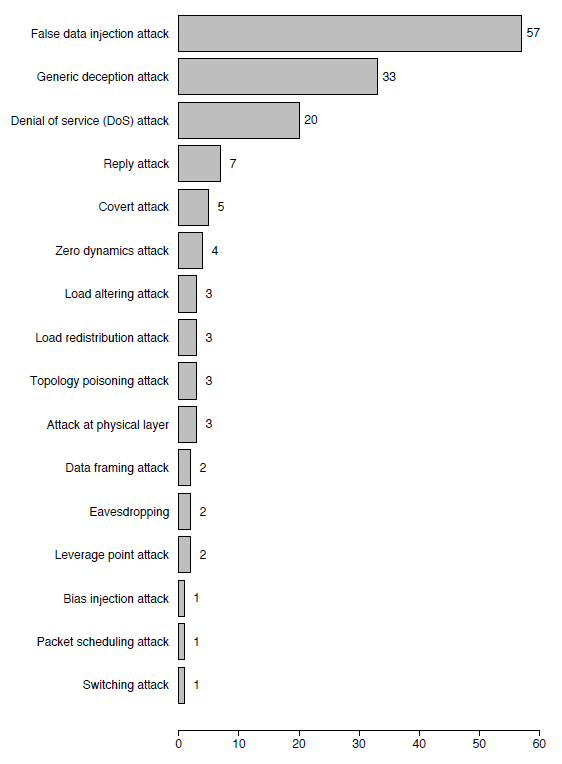
\includegraphics[width=0.5\linewidth]{img1.png}
        \end{figure}
    \end{center}
\end{frame}

\subsection{Caso di studio}
\begin{frame}{Caso di studio: dispositivi medici impiantabili}
    I moderni IMD comunicano in modalità wireless con un dispositivo esterno detto \textit{programmer} e inviano dati per monitorare e ricevere la migliore 
    terapia per il paziente. 
    
    Utili per monitorare i parametri vitali del paziente, soprattutto se in condizioni critiche.

    \begin{center}
        \begin{figure}[H]
          \centering
          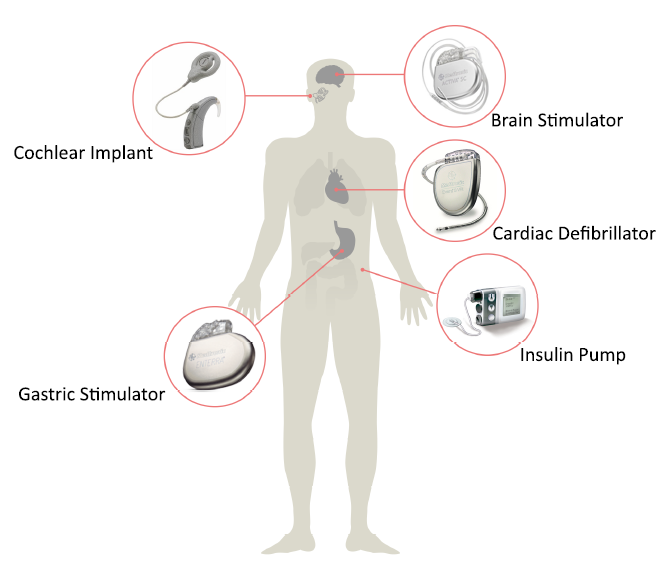
\includegraphics[width=0.5\linewidth]{img2.png}
        \end{figure}
    \end{center}
\end{frame}

\begin{frame}{Attacchi ai IMD}
    I principali attacchi ai dispositivi medici impiantabili sono:
    \begin{itemize}
        \item \textbf{Information Harvesting}: se nessun meccanismo di autenticazione è applicato nell'IMD, l'avversario può ottenere informazioni 
        riservate sulla salute del paziente oppure ascoltare le comunicazioni tra dispositivo e programmer per utilizzarle in ulteriori attacchi. 
        \item \textbf{Tracking the patient}: la comunicazione wireless può essere facilmente rilevata, soprattutto se si è all'aperto. L'attaccante 
        può tracciare il movimento del paziente comportando una grave violazione della privacy.        
    \end{itemize}
\end{frame}

\begin{frame}{Attacchi ai IMD}
    \begin{itemize}
        \item \textbf{Impersonation}: se il canale wireless non è sufficientemente protetto, l'avversario può origliare comunicazioni e registrare
        la risposta dell'IMD. 
        Utilizzati per raccogliere informazioni riguardo terapie e alimentazione del paziente e ritardare la risposta del medico curante ai bisogni del 
        paziente.
        \item \textbf{Relaying}: l'IMD viene ingannato facendogli presumere che il programmer sia vicino ad esso. L'attaccante utilizza due device 
        chiamati \textit{ghost} e \textit{leech} che impersonificano rispettivamente l'IMD e il programmer. In questo modo continuano a 
        trasmettere i messaggi tra IMD e programmer ingannando l'IMD  e facendogli credere di parlare con un programmer lecito.
    \end{itemize}
\end{frame}

\begin{frame}{Attacchi ai IMD}
    \begin{itemize}
        \item \textbf{Denial of Service}: si vuole manomettere la capacità dell'IMD di svolgere il proprio lavoro: 
            \begin{itemize}
                \item Richiedere attività che consumano l'energia del dispositivo - \textit{Power draining attack};
                \item Interferire nella comunicazione con il servizio di manutenzione;
                \item Far spegnere il dispositivo applicando un campo magnetico in prossimità del paziente.
            \end{itemize}
    \end{itemize}
\end{frame}


\section{Metodi di difesa}
\begin{frame}{Difesa}
    La strategia di difesa si può classificare in:
    \begin{itemize}
        \item \textbf{Prevenzione}: riduzione della vulnerabilità del sistema. Riguarda tutte le operazioni eseguite \textit{offline} prima che il sistema venga 
        perturbato o attaccato;
        \item \textbf{Rilevazione}: operazioni eseguite \textit{online}, quando un attacco si verifica. Il sistema viene costantemente monitorato per rilevare
        eventuali attacchi. L'attacco, se rilevato, viene isolato e vengono identificati i componenti compromessi;
        \item \textbf{Mitigazione}: interrompere e neutralizzare l'attacco e cercare di ridurne l'impatto.
    \end{itemize}
    
\end{frame}


\end{document}
